\section{Paradigma Lógico}

\subsection{Características generales}

\begin{itemize}
  \item Se basa en el uso de la lógica como un lenguaje de programación: los programas son predicados.
  \item La computación se expresa a través de ``proof search''. Para esto, se especifican ciertos \xbf{hechos} y \xbf{reglas}, así como un objetivo o \xbf{goal} a probar. Luego, un motor de inferencia trata de probar que el objetivo es consecuencia de los hechos y reglas.
  \item No hay un estado global.
  \item Los resultados intermedios son pasados a través de unificación.
  \item Repetición basada en recursión.
  \item Tiene un \xbf{alto nivel de abstracción}: tiende a ser una \xit{especificación ejecutable}.
  \item Es \xbf{declarativo}: la máquina se encarga de buscar el \xit{cómo} y nosotros elegimos el \xit{qué}.
  \item Fundamento lógico robusto. Utiliza técnicas de \xit{Resolución}.
  \item Ejecución lenta en comparación con otros paradigmas.
\end{itemize}

\subsection{Repaso lógica proposicional}

\paragraph{Sintaxis}

Dado un conjunto $\mathcal{V}$ de variables proposicionales, definimos inductivamente el conjunto de formulas proposicionales de la siguiente manera:

\begin{itemize}
  \item Una variable proposicional $P_0, P_1, \dots$ es una proposición.
  \item Si $A, B$ son proposiciones, entonces:
    \begin{itemize}
      \item $\lnot A$ es una proposición.
      \item $A \land B$ es una proposición.
      \item $A \lor B$ es una proposición.
      \item $A \supset B$ es una proposición.
      \item $A \iff B$ es una proposición.
    \end{itemize}
\end{itemize}

\paragraph{Semántica}

Una \xbf{valuación} es una función $v:\mathcal{V}\to\{T,F\}$ que asigna valores de verdad a las variables proposicionales.

Una valuación \xbf{satisface} una proposición $A$ si $v \models A$ donde

\begin{align*}
  v \models P &\text{ sii } v(P) = T \\
  v \models \lnot A &\text{ sii } v \not\models A \text{ (que es lo mismo que $\lnot v \models A$)} \\
  v \models A \land B &\text{ sii } v \models A \text{ y } v \models B \\
  v \models A \lor B &\text{ sii } v \models A \text{ o } v \models B \\
  v \models A \supset B &\text{ sii } v \not\models A \text{ o } v \models B \\
  v \models A \iff B &\text{ sii } (v \models A \text{ sii } v \models B) \\
\end{align*}

\paragraph{Tautologías y satisfacibilidad}

Una proposición $A$ es:
\begin{itemize}
  \item Una tautología si $v \models A$ para toda valuación $v$.
  \item Satisfacible si existe una valuación $v$ tal que $v \models A$.
  \item Insatisfacible si no es satisfacible.
\end{itemize}

Un conjunto de proposiciones $S$ es
\begin{itemize}
  \item Satisfacible si existe una valuación $v$ tal que para todo $A \in S$, se tiene $v \models A$.
  \item Insatisfacible si no es satisfacible.
\end{itemize}

\begin{teo}
  Una proposición $A$ es una tautología sii $\lnot A$ es insatisfacible.
\end{teo}
\begin{proof}
  \hspace{0.5em}\\
  $\implies$. Si $A$ es tautología, para toda valuación $v$, $v \models A$. Entonces $v \not\models \lnot A$.\\
  $\Longleftarrow$. Si $\lnot A$ es insatisfacible, para toda valuación $v$, $v \not\models \lnot A$. Entonces $v \models A$.
\end{proof}

\paragraph{Forma Normal Conjuntiva (FNC)}

Un literal es una variable proposicional $P$ o su negación $\lnot P$.

Una proposición $A$ está en FNC si es una conjunción

\[C_1 \land \dots \land C_n\]

donde cada $C_i$ (llamado cláusula) es una disyunción

\[B_{i1} \lor \dots \lor B_{in}\]

y cada $B_{ij}$ es un literal.

Entonces, una FNC es una \xit{conjunción de disyunciones de literales}.

\begin{teo}
  Para toda proposición $A$ puede hallarse una proposición $A'$ en FNC que es lógicamente equivalente a $A$.
\end{teo}

\paragraph{Notación conjuntista para FNC}

Dado que tanto $\lor$ como $\land$
\begin{itemize}
  \item Son conmutativos.
  \item Son asociativos.
  \item Son idempotentes.
\end{itemize}

Podemos asumir que
\begin{itemize}
  \item Cada cláusula $C_i$ es distinta.
  \item Cada cláusula puede verse como un conjunto de literales distintos.
\end{itemize}

Consecuentemente, para una FNC podemos usar la notación

\[\{C_1, \dots, C_n\}\]

donde cada $C_i$ es un conjunto de literales

\[\{B_{i1}, \dots, B_{in}\}\]

\subsection{Método de resolución para lógica proposicional}

El método de \xbf{Resolución} fue introducido en 1965 y se basa en el principio de demostración por refutación: probar que $A$ es válido mostrando que $\lnot A$ es insatisfacible.

Además, se basa en el hecho que el conjunto del conjunto de cláusulas

\[\{C_1, \dots, C_m, \{A,P\}, \{B, \lnot P\}\}\]

es lógicamente equivalente a

\[\{C_1, \dots, C_m, \{A,P\}, \{B, \lnot P\}, \{A,B\}\}\]

En consecuencia, el conjunto de cláusulas

\[\{C_1, \dots, C_m, \{A,P\}, \{B, \lnot P\}\}\]

es insatisfacible sii

\[\{C_1, \dots, C_m, \{A,P\}, \{B, \lnot P\}, \{A,B\}\}\]

es insatisfacible.

Las cláusula $\{A,B\}$ se llama resolvente de las cláusulas $\{A, P\}$ y $\{B, \lnot P.\}$. El resolvente de las cláusulas $\{P\}$ y $\{\lnot P\}$ es la cláusula vacía y se anota $\square$.

Entonces, la regla de resolución nos queda:

\[\resol{\{A_1,\dots,A_m,Q\}\ \{B_1,\dots,B_n,\lnot Q\}}{\{A_1,\dots,A_m, B_1,\dots,B_n\}}\]

En el método de resolución, cada \xbf{paso de resolución} consiste en agregar a un conjunto $S$ la resolvente $C$ de dos cláusulas $C_1, C_2$ que pertenecen a $S$ (asumimos que $C$ no pertenecía a $S$). Lo importante es que cada paso de resolución preserva la insatisfacibilidad, por lo que $S$ es insatisfacible sii $S \cup \{C\}$ es insatisfacible.

Por último, un conjunto de cláusulas se llama una \xbf{refutación} si contiene a la cláusula vacía ($\square$), que es insatisfacible.

El método de resolución trata de construir una secuencia de conjuntos de cláusulas, obtenidas usando pasos de resolución hasta llegar a una refutación.

\[S_1 \implies S_2 \implies \dots \implies S_n \ni \square\]

Con lo cual, se sabe que el conjunto inicial de cláusulas es insatisfacible.

\paragraph{Terminación de la regla de resolución}

La aplicación reiterada de esta regla siempre termina (suponiendo que cada resolvente que se agrega es nuevo). Esto se puede ver ya que:

\begin{itemize}
  \item El resolvente se forma con los literales distintos que aparecen en el conjunto de cláusulas de partida $S$.
  \item Hay una cantidad finita de literales en el conjunto de cláusulas de partida $S$.
\end{itemize}

\begin{teo}
  Dado un conjunto finito $S$ de cláusulas, $S$ es insatisfacible sii tiene una refutación.
\end{teo}

\paragraph{Recapitulando}

Para probar que $A$ es una tautología:
\begin{enumerate}
  \item Calculamos la FNC de $\lnot A$
  \item Aplicamos el método de resolución.
  \item Si hallamos una refutación, $\lnot A$ es insatisfacible, y por lo tanto $A$ es una tautología.
  \item Si no, $\lnot A$ es satisfacible, y por lo tanto $A$ no es una tautología.
\end{enumerate}

\subsection{Repaso lógica de primer orden}

\paragraph{Sintaxis}

Un lenguaje de primer orden $\mathcal{L}$ consiste en:

\begin{itemize}
  \item Un conjunto numerable de constantes $c_0, c_1, \dots$
  \item Un conjunto numerable de símbolos de función con aridad $n > 0$, $f_0, f_1, \dots$
  \item Un conjunto numerable de símbolos de predicado con aridad $n \geq 0$, $P_0, P_1, \dots$.
\end{itemize}

Sea $\mathcal{V}$ un conjunto numerable de variables. El conjunto de $\mathcal{L}$-términos se define inductivamente como:
\begin{itemize}
  \item Toda constante de $\mathcal{L}$ y toda variable es un $\mathcal{L}$-término
  \item Si $t_1,\dots,t_n \in \mathcal{L}$-términos y $f$ es un símbolo de función de aridad $n$, entonces $f(t_1,\dots,t_n) \in \mathcal{L}$-términos
\end{itemize}

El conjunto de $\mathcal{L}$-fórmulas atómicas se define inductivamente como:
\begin{itemize}
  \item Todo símbolo de predicado de aridad 0 es una $\mathcal{L}$-fórmula atómica
  \item Si $t_1,\dots,t_n \in \mathcal{L}$-términos y $P$ es un símbolo de predicado de aridad $n$, entonces $P(t_1,\dots,t_n) \in \mathcal{L}$-fórmulas atómicas
\end{itemize}

El conjunto de $\mathcal{L}$-fórmulas se define inductivamente como:
\begin{itemize}
  \item Toda $\mathcal{L}$-fórmula atómica es una $\mathcal{L}$-fórmula
  \item Si $A,B \in \mathcal{L}$-fórmulas, entonces $(A \land B)$, $(A \lor B)$, $(A \supset B)$, $(A \iff B)$ y $\lnot A$ son $\mathcal{L}$-fórmulas
  \item Para toda variable $x_i$ y cualquier $\mathcal{L}$-fórmula $A$, $\forall x_i.A$ y $\exists x_i.A$ son $\mathcal{L}$-fórmulas
\end{itemize}

Las variables pueden ocurrir libres o ligadas. Los cuantificadores ligan variables. Usamos $FV(A)$ y $BV(A)$ para referirnos a las variables libres y ligadas respectivamente de $A$.

Una fórmula $A$ se dice \xbf{rectificada} si
\begin{itemize}
  \item $FV(A)$ y $BV(A)$ son disjuntos y
  \item Cuantificadores distintos de $A$ ligan variables distintas.
\end{itemize}

Toda fórmula se puede rectificar (renombrando variable ligadas) a una fórmula lógica equivalente. Una sentencia es una fórmula cerrada (sin variables libres).

\paragraph{Semántica}

Dado un lenguaje de primer orden $\mathcal{L}$, una estructura para $\mathcal{L}$ es un par $(M,I)$ donde
\begin{itemize}
  \item $M$ (dominio) es un conjunto no vacío.
  \item $I$ (función de interpretación) asigna funciones y predicados sobre $M$ a símbolos de $\mathcal{L}$ de la siguiente manera:
  \begin{enumerate}
    \item Para toda constante $c$, $I(c) \in M$
    \item Para toda función $f$ de aridad $n > 0$, $I(f): M^n \to M$
    \item Para todo predicado $P$ de aridad $n \geq 0$, $I(P) : M^n \to \{T,F\}$
  \end{enumerate}
\end{itemize}

Sea $(M,I)$ una estructura para $\mathcal{L}$. Una asignación es una función $s:\mathcal{V} \to M$, y la relación $s \models_{(M,I)} A$ establece que la asignación $s$ satisface la fórmula $A$ en la estructura $(M,I)$.

Entonces,
\begin{itemize}
  \item Una fórmula $A$ es satisfacible en $(M,I)$ sii existe una asignación $s$ tal que $s \models_{(M,I)} A$.
  \item Una fórmula $A$ es satisfacible sii existe una estructura $(M,I)$ tal que $A$ es satisfacible en $(M,I)$.
  \item Una fórmula $A$ es válida en $(M,I)$ sii $s \models_{(M,I)} A$, para toda asignación $s$.
  \item Una fórmula $A$ es válida sii es válida en toda estructura $(M,I)$.
  \item Luego, $A$ es válida sii $\lnot A$ es insatisfacible.
\end{itemize}

\begin{teo}[Teorema de Church]
  No existe un algoritmo que pueda determinar si una fórmula de primer orden es válida.

  Como consecuencia, el método de resolución que mostramos no es un procedimiento efectivo, sino que es un algoritmo de semi-decision:
  \begin{itemize}
    \item Si una sentencia es insatisfacible hallará una refutación,
    \item Pero si es satisfacible puede que no se detenga.
  \end{itemize}
\end{teo}

\subsection{Método de resolución para lógica de primer orden}

Cuando trabajamos en lógica de primer orden también tenemos una FNC en notación de conjuntos, Forma clausal, pero requiere tener en cuenta los cuantificadores ($\forall$ y $\exists$). Podemos llevar una fórmula de primer orden a Forma clausal con los siguientes pasos:

\begin{enumerate}
  \item \xbf{Eliminar implicaciones}.
  \item \xbf{Pasar a Forma normal negada}.
  \item \xbf{Pasar a Forma normal prenexa (opcional)}.
  \item \xbf{Pasar a Forma normal de Skolem (puede hacerse antes que el paso anterior)}.
  \item \xbf{Pasar a Forma normal conjuntiva}.
  \item \xbf{Distribuir cuantificadores universales}.
\end{enumerate}

Todos estos pasos preservan validez lógica, salvo la \xit{Skolemización}, que preserva satisfacibilidad.
Vamos cada paso en detalle.

\paragraph{Eliminar implicaciones}

Consiste en escribir la fórmula en términos de $\land, \lor, \lnot, \forall, \exists$.

\paragraph{Forma normal negada (FNN)}

Se define inductivamente como:
\begin{itemize}
  \item Para cada fórmula atómica $A$, $A$ y $\lnot A$ están en FNN.
  \item Si $A, B \in$ FNN entonces $(A \land B), (A \lor B) \in$ FNN.
  \item Si $A \in$ FNN, entonces $\forall x.A, \exists x.A \in$ FNN.
\end{itemize}

Y podemos definir las siguientes reglas para hacer el pasaje más sencillo:
\begin{itemize}
  \item $\lnot (A \land B)$ pasa a $(\lnot A \lor \lnot B)$
  \item $\lnot (A \lor B)$ pasa a $(\lnot A \land \lnot B)$
  \item $\lnot\lnot A$ pasa a $A$
  \item $\lnot\forall x.A$ pasa a $\exists x.\lnot A$
  \item $\lnot\exists x.A$ pasa a $\forall x.\lnot A$
\end{itemize}

\paragraph{Forma normal prenexa}

Consiste en pasar todos los cuantificadores ($\forall$ y $\exists$) al principio de la fórmula. También contamos con reglas para ayudar a hacer el pasaje:
\begin{itemize}
  \item $(\forall x.A) \land B$ pasa a $\forall x. (A \land B)$
  \item $(A \land \forall x.B)$ pasa a $\forall x. (A \land B)$
  \item $(\exists x.A) \land B$ pasa a $\exists x. (A \land B)$
  \item $(A \land \exists x.B)$ pasa a $\exists x. (A \land B)$
  \item $(\forall x.A) \lor B$ pasa a $\forall x. (A \lor B)$
  \item $(A \lor \forall x.B)$ pasa a $\forall x. (A \lor B)$
  \item $(\exists x.A) \lor B$ pasa a $\exists x. (A \lor B)$
  \item $(A \lor \exists x.B)$ pasa a $\exists x. (A \lor B)$
\end{itemize}

\paragraph{Forma normal de Skolem}

El objetivo de este paso es
\begin{itemize}
  \item Eliminar los cuantificadores existenciales ($\exists$)
  \item Sin alterar la satisfacibilidad (y por lo tanto la insatisfacibilidad).
\end{itemize}

Para esto, introducimos \xit{testigos} (parámetros), tal que:
\begin{itemize}
  \item Todo cuantificador existencial se reemplaza por una constante o función de Skolem. Ejemplo $\exists x. P(x)$ pasa a $P(c)$, con $c$ una nueva constante.
  \item Cada ocurrencia de una subfórmula $\exists x. B$ se reemplaza en la fórmula $A$ por $B\{x \from f(x_1, \dots, x_n)\}$, donde $f$ es un símbolo de función nuevo y las $x_1, \dots, x_n$ son las variables de las que depende $x$ en $B$. Por ejemplo $\forall x.\exists y. P(x,y)$ pasa a $\forall x. P(x, g(x))$.
\end{itemize}

\xit{Nota}: no es posible eliminar los cuantificadores existenciales sin alterar la validez. Ejemplo: $\exists x. (P(a) \supset P(x))$ es válida pero $P(a) \supset P(b)$ no lo es.

La forma normal de Skolem de $A$ (escrito como $SK(A)$) se puede definir recursivamente. Sea $A'$ cualquier subfórmula de $A$:
\begin{itemize}
  \item Si $A'$ es una fórmula atómica o su negación, $SK(A') = A'$.
  \item Si $A'$ es de la forma $(B \star C)$ con $\star \in \{\land, \lor\}$, entonces $SK(A') = (SK(B) \star SK(C))$.
  \item Si $A'$ es de la forma $\forall x.B$, entonces $SK(A') = \forall x.SK(B)$.
  \item Si $A'$ es de la forma $\exists x.B$ y $\{x, y_1, \dots, y_m\}$ son las variables libres de B (que se ligan en $A$, dado que $A$ es sentencia), entonces
    \begin{itemize}
      \item Si $m > 0$, crear un nuevo símbolo de función de Skolem, $f_x$ de aridad $m$ y definir $SK(A') = SK(B\{x \from f_x(y_1, \dots, y_m)\})$
      \item Si $m = 0$, crear una nueva constante de Skolem $c_x$ y definir $SK(A') = SK(B\{x \from c_x\})$
    \end{itemize}
    Notar que dado que $A$ está rectificada, cada $f_x$ y $c_x$ es única.
\end{itemize}

\xit{Tip}: siempre conviene skolemizar de afuera hacia adentro, para evitar cambios innecesarios.

\paragraph{Forma normal conjuntiva (FNC)}

Este paso es idéntico a como hacíamos cuando estábamos trabajando con fórmulas proposicionales. Llevamos la fórmula a la forma

\[C_1 \land \dots \land C_r\]

 donde cada $C_i$ es una disyunción de literales.

\paragraph{Distribuir cuantificadores universales}

Consiste en distribuir los cuantificadores sobre cada conjunción usando la fórmula válida $\forall x.(A\land B) \iff \forall x. A \land \forall x. B$ arrojando una conjunción de cláusulas

\[\forall x_1,\dots,x_n C_1 \land \dots \land \forall x_1,\dots,x_m C_r\]

 donde cada $C_i$ es una disyunción de literales.

Por último, lo simplificamos escribiendo $\{C_1, \dots, C_r\}$

\paragraph{Regla de resolución para lógica de primer orden}

Ahora que tenemos nuestra fórmula correctamente en Forma Clausal veamos cómo hacemos para aplicar resolución.

Como motivación, consideremos la fórmula $(\forall x. P(x)) \land \lnot P(a)$, que claramente es insatisfacible. Sin embargo, no podemos aplicar la regla de resolución estandar, ya que $P(x)$ y $P(a)$ no son idénticos\dots\ pero sí son unificables.

Definimos una nueva regla de resolución, como

\[\resol{\{B_1,\dots,B_k,A_1,\dots,A_m\}\ \{\lnot D_1,\dots,\lnot D_j,C_1,\dots,C_n\}}{\sigma(\{A_1,\dots,A_m, C_1,\dots,C_n\})}\]

donde $\sigma$ es el MGU de $\{B_1,\dots,B_k, D_1,\dots,D_j\}$. Algunas observaciones:
\begin{itemize}
  \item Asumimos que las cláusulas $\{B_1,\dots,B_k,A_1,\dots,A_m\}$ y $\{\lnot D_1,\dots,\lnot D_j,C_1,\dots,C_n\}$ no tienen variables en común; en caso contrario se renombran las variables.
  \item Notar que $\sigma(B_1) = \dots = \sigma(B_k) = \sigma(D_1) = \dots = \sigma(D_j) $
  \item La cláusula $\sigma(\{A_1,\dots,A_m, C_1,\dots,C_n\})$ se llama resolvente, igual que antes.
\end{itemize}

Análogamente al caso proposicional, tenemos las nociones de cláusula vacía, paso de resolución y refutación. Además, tenemos el siguiente resultado.

\begin{teo}[Teorema de Herbrand-Skolem-Gödel]
  Cada paso de resolución en lógica de primer orden preserva satisfacibilidad.
\end{teo}

\paragraph{Regla de resolución binaria}

Incorpora una regla adicional que es útil en algunos casos: \xit{factorización}

\[\resol{\{B_1,\dots,B_k,A_1,\dots,A_m\}}{\sigma(\{B_1,A_1,\dots,A_m\})}\]

donde $\sigma$ es el MGU de $\{B_1,\dots,B_k\}$.

\subsection{Resolución lineal}

Si bien el método de resolución general es completo, hallar refutaciones es un proceso muy caro en el caso general ya que el espacio de búsqueda producido puede ser enorme. Además, hay un alto grado de no-determinismo.
\begin{itemize}
  \item ¿Qué cláusulas elegimos? Hace falta una Regla de búsqueda.
  \item ¿Qué literales eliminamos? Hace falta una Regla de selección.
\end{itemize}

Estas reglas ayudan a reducir el espacio de búsqueda, y es deseable que estas restricciones no renuncien a la completitud del método.

Una secuencia de pasos de resolución a partir de $S$ es \xbf{lineal} si es de la forma:

\begin{center}
  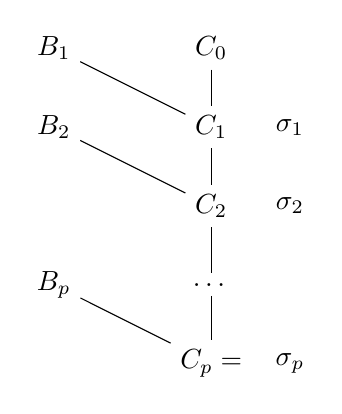
\begin{tikzpicture}
      \tikzstyle{ann} = [draw=none,fill=none,right]
      \node[draw=none, fill=none] (C0) at (0,0) {$C_0$};
      \node[draw=none, fill=none] (B1) at (-2,0) {$B_1$};
      \node[draw=none, fill=none] (C1) at (0,-1) {$C_1$};
      \node[draw=none, fill=none] (s1) at (1,-1) {$\sigma_1$};
      \node[draw=none, fill=none] (B2) at (-2,-1) {$B_2$};
      \node[draw=none, fill=none] (C2) at (0,-2) {$C_2$};
      \node[draw=none, fill=none] (s2) at (1,-2) {$\sigma_2$};
      \node[draw=none, fill=none] (aux) at (0,-3) {\dots};
      \node[draw=none, fill=none] (Bp) at (-2,-3) {$B_p$};
      \node[draw=none, fill=none] (Cp) at (0,-4) {$C_p = \square$};
      \node[draw=none, fill=none] (sp) at (1,-4) {$\sigma_p$};
      \path [-](B1) edge node {} (C1);
      \path [-](C0) edge node {} (C1);
      \path [-](B2) edge node {} (C2);
      \path [-](C1) edge node {} (C2);
      \path [-](C2) edge node {} (aux);
      \path [-](Bp) edge node {} (Cp);
      \path [-](aux) edge node {} (Cp);
  \end{tikzpicture}
\end{center}

donde $C_0$ y cada $B_i$ es un elemento de $S$ o algún $C_j$ con $j < i$. Es decir, para cada nuevo paso de resolución tengo que usar el último resolvente que generé y algún elemento de $S$.

Observaciones de la resolución lineal:
\begin{itemize}
  \item En general, reduce el espacio de búsqueda considerablemente.
  \item Preserva completitud.
  \item Sin embargo, sigue siendo altamente no-determinístico.
\end{itemize}

\subsection{Cláusulas de Horn}

Es un tipo de subclase de fórmulas para las cuales existen procesos eficientes para producir refutaciones sin perder completitud.

Una cláusula de Horn es una disyunción de literales que tiene \xit{a lo sumo} un literal positivo. Para conjuntos de cláusulas de Horn se puede usar la resolución SLD, que tiene buenas propiedades.

Dividimos estas cláusulas en 3 grupos:
\begin{itemize}
  \item \xit{Goal}: todos los literales negativos.
  \item \xit{Definición}: tiene exactamente un literal positivo. Puede ser:
    \begin{itemize}
      \item \xit{Regla}: un literal positivo, y todos los demás negativos.
      \item \xit{Hecho}: sólo un literal positivo.
    \end{itemize}
\end{itemize}

Tener en cuenta que no todas las fórmulas de primer orden pueden expresarse como una cláusula de Horn, aunque es lo suficientemente expresivo para representar programas

\subsection{Resolución SLD}

Es una variante de la resolución lineal.

Sea $S = P \cup \{G\}$ un conjunto de cláusulas de Horn (con nombres de variables disjuntos) tal que
\begin{itemize}
  \item $P$ es un conjunto de cláusulas de definición y
  \item $G$ es una cláusula \xit{goal} o negativa.
\end{itemize}

Decimos que $S$ son las cláusulas de entrada. $P$ se conoce como el programa o base de conocimientos y $G$ es el objetivo o meta.

Luego, una secuencia de pasos de resolución SLD para $S$ es una secuencia $\langle N_0, \dots, N_p \rangle$ de cláusulas negativas que satisfacen:
\begin{itemize}
  \item $N_0$ es el goal $G$.
  \item Para todo $N_i$ en la secuencia, $0 < i < p$, si $N_i$ es
  \[\lnot A_1,\dots,\lnot A_{k-1},\lnot A_k,\lnot A_{k+1},\dots,\lnot A_n\]
  entonces hay alguna cláusula de definición $C_i$ de la forma $\{A, \lnot B_1,\dots, \lnot B_m\}$ en $P$ tal que $A_k$ y $A$ son unificables con MGU $\sigma$, y si
    \begin{itemize}
      \item $m = 0$, entonces $N_{i+1}$ es $\{\sigma(\lnot A_1,\dots,\lnot A_{k-1},\lnot A_{k+1},\dots,\lnot A_n)\}$
      \item $m > 0$, entonces $N_{i+1}$ es $\{\sigma(\lnot A_1,\dots,\lnot A_{k-1}, \lnot B_1,\dots, \lnot B_m, \lnot A_{k+1},\dots,\lnot A_n)\}$
    \end{itemize}
\end{itemize}

En el caso de que $\langle N_0, \dots, N_p \rangle$ sea una refutación, entonces $N_p = \square$. Y por ser lineal, tiene que tener la forma:

\begin{center}
  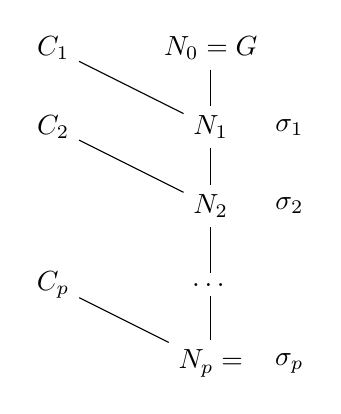
\begin{tikzpicture}
      \tikzstyle{ann} = [draw=none,fill=none,right]
      \node[draw=none, fill=none] (N0) at (0,0) {$N_0 = G$};
      \node[draw=none, fill=none] (C1) at (-2,0) {$C_1$};
      \node[draw=none, fill=none] (N1) at (0,-1) {$N_1$};
      \node[draw=none, fill=none] (s1) at (1,-1) {$\sigma_1$};
      \node[draw=none, fill=none] (C2) at (-2,-1) {$C_2$};
      \node[draw=none, fill=none] (N2) at (0,-2) {$N_2$};
      \node[draw=none, fill=none] (s2) at (1,-2) {$\sigma_2$};
      \node[draw=none, fill=none] (aux) at (0,-3) {\dots};
      \node[draw=none, fill=none] (Cp) at (-2,-3) {$C_p$};
      \node[draw=none, fill=none] (Np) at (0,-4) {$N_p = \square$};
      \node[draw=none, fill=none] (sp) at (1,-4) {$\sigma_p$};
      \path [-](C1) edge node {} (N1);
      \path [-](N0) edge node {} (N1);
      \path [-](C2) edge node {} (N2);
      \path [-](N1) edge node {} (N2);
      \path [-](N2) edge node {} (aux);
      \path [-](Cp) edge node {} (Np);
      \path [-](aux) edge node {} (Np);
  \end{tikzpicture}
\end{center}

Observaciones de la resolución SLD:
\begin{itemize}
  \item No se especifica regla de búsqueda ni de selección.
  \item La sustitución respuesta es $\sigma_p \circ \dots \circ \sigma_2 \circ \sigma_1$
  \item \xbf{Corrección:} Si un conjunto de cláusulas de Horn tiene refutación SLD, entonces es insatisfacible.
  \item \xbf{Completitud:} Dado un conjunto de cláusulas de Horn $P \cup \{G\}$ tal como se describió, si $P \cup \{G\}$ es insatisfacible, existe una refutación SLD cuya primera cláusula es $G$.
\end{itemize}

\subsection{Prolog}

Es un lenguaje de programación lógico presentado en el año 1971. Los programas se escriben en un subconjunto de la lógica de primer orden, y el mecanismo teórico en el que se basa es el método de resolución.

En particular, utilizar resolución SLD con las siguientes restricciones:
\begin{itemize}
  \item \xbf{Regla de búsqueda:} se seleccionan las cláusulas de programa de arriba hacia abajo, en el orden en que fueron introducidas.
  \item \xbf{Regla de selección:} seleccionar el átomo de más a la izquierda.
\end{itemize}

Estas dos reglas se definen como la \xit{estrategia}. Cada estrategia determina un árbol de búsqueda o árbol SLD.

Dado que $(A_1 \land \dots \land A_n) \supset B \iff \lnot (A_1 \land \dots \land A_n) \lor B \iff \lnot A_1 \lor \dots \lor \lnot A_n \lor B$, tenemos que las cláusulas $P$ en Prolog se escriben
\begin{itemize}
  \item \xtt{B :- A\_1, \dots, A\_n.} para $\{B, \lnot A_1, \dots, \lnot A_n\}$ (reglas)
  \item \xtt{B.} para $\{B\}$ (hechos)
\end{itemize}

\paragraph{Búsqueda de refutaciones SLD en Prolog}
\begin{itemize}
  \item Recorre el árbol SLD en profundidad (\xbf{DFS}), lo cual permite implementarlo de manera muy \xit{eficiente}:
  \begin{itemize}
    \item Se usa una pila para representar los átomos del goal.
    \item Se hace un push del resolvente del átomo del tope de la pila con la cláusula de definición.
    \item Se hace un pop cuando el átomo del tope de la pila no unifica con ninguna cláusula de definición más (luego, el átomo que queda en el tope se unifica con la siguiente cláusula de definición).
  \end{itemize}
  \item \xbf{Desventaja:} puede no llegar a encontrar una refutación SLD aún si existe.
\end{itemize}

\paragraph{Operador Cut}

Es una anotación que permite poder el árbol SLD, y se encuentra presente por cuestiones de eficiencia. En Prolog se escribe el símbolo \xtt{!}.

\begin{itemize}
  \item Cuando se selecciona un cut, tiene éxito inmediatamente.
  \item Si, debido a backtracking, se vuelve a este cut, su efecto es el de hacer fallar el goal que le dio origen. De esta forma, forzamos determinismo (a lo sumo una solución).
  \item En particular, todas las variables que estaban ligadas al momento de pasar por el cut, quedan ligadas por el resto de la ejecución del programa y no pueden cambiarse.
\end{itemize}

\paragraph{Operador Not (negación por falla)}

Antes veamos algunas definiciones:

\begin{itemize}
  \item Decimos que un árbol SLD \xbf{falla finitamente} si es finito y no tiene ramas de éxito.
  \item Dado un programa $P$, definimos el \xbf{conjunto de falla finita} de $P$ como \{$B$ | $B$ átomo cerrado ('ground') y existe un árbol SLD que falla finitamente con  $B$ como raíz \}
\end{itemize}

Entonces, la \xbf{negación por falla} se define como:

\[\resol{B \text{ átomo cerrado}\quad B \text{ en conjunto de falla finita de } P}{\lnot B}\]

El operador \xtt{not} nos permite utilizar la negación por falla y se define como:

\begin{lstlisting}[language=Prolog]
not(G) :- call(G), !, fail.
not(G).
\end{lstlisting}

La clave está en combinar el operador \xtt{!} y \xtt{fail}. Una vez que el \xtt{Goal} tiene éxito, el cut nos prohíbe volver atrás en el árbol SLD, y el \xtt{fail} hace que la solución actual falle. Como no hay más ramas que explorar, toda la consulta falla.

Notar que es distinto a la negación lógica. Si la cláusula no es cerrada, \xtt{not(G)} tiene éxito si no existe \xit{ninguna} valuación tal que \xtt{G} se satisface.

Además, observar que el \xtt{not(G)} nunca instancia variables de \xtt{G}:
\begin{itemize}
  \item Si \xtt{G} tiene éxito, \xtt{fail} falla y descarta la sustitución.
  \item Caso contrario, \xtt{not(G)} tiene éxito inmediatamente (sin afectar \xtt{G}).
\end{itemize}
